%| report template for CSUS Senior Design
%|
%| language: LaTeX
%| Author: Ben Smith
%| 
%| This source has been tagged with the "#CHANGE" tag in areas
%| that require updating when making a new docuent
%|
%| This source will generate a PDF file complete with thumbnails navigation menu and metadata,
%| 

\documentclass[12pt,article]{IEEEtran}
%| This section will essentially create variables to be used in some
%| of the documents formatting and the PDF's metadata 
%|
\newcommand{\TITLE}{Design Document}
\newcommand{\KEYWORDS}{Electrical Assist, FPGA, Electric Speed Controller, Bicycle.}
\newcommand{\ABSTRACT}{This document contains the featureset for our proposed smart electrical bicycle.
Also contains descriptions of our features, the resources needed to implement them, and the estimated 
time required to develop the system.}
\newcommand{\AUTHOR}{Micheal Frith, David Larribas, Devin Moore, Benjamin Smith}
\newcommand{\DUEDATE}{September 10, 2013}
%| =================================================================================================
%| Formatting options
%| =================================================================================================

%| Enables PDF metadata, thumbnails, and navigation
\newcommand\MYhyperrefoptions{
    bookmarks=true,
    bookmarksnumbered=true,
    bookmarksopen=true,
    bookmarkstype={toc},
    pdfpagemode={UseOutlines},
    plainpages=false,
    pdfpagelabels=true,
    colorlinks=true,
    linkcolor={black},
    citecolor={black},
    pagecolor={black},
    urlcolor={black},
    final=true,
    pdftex,
    pdftitle={\TITLE},                                                          
    pdfsubject={\ABSTRACT},                                             
    pdfauthor={Micheal Frith, David Larribas, Devin Moore, Benjamin Smith},             
    pdfkeywords={\KEYWORDS}}                                        

%| Calls hyper ref package 
\usepackage[\MYhyperrefoptions]{hyperref}
%| Override compsoc class' Palatino font for body text, restores to Times New Roman
\renewcommand{\rmdefault}{ptm}\selectfont

%| IEEE Citation package
\usepackage{cite}

%| American Mathematical Society package for fancy maths    
\usepackage[cmex10]{amsmath}
\interdisplaylinepenalty=2500               % Restores IEEE line spacing after amsmath

%| For importing PDF pages
\usepackage[ options ]{pdfpages}

%| Better tables than LaTeX 2e
\usepackage{array}

%| Improved URL handling
\usepackage{url}

% correct bad hyphenation here
\hyphenation{op-tical net-works semi-conduc-tor}

%for placing graphics
\usepackage{graphicx}

%| for static table placement
\usepackage{float}
\restylefloat{table}

\begin{document}

%| Inserts header cover sheet 
\begin{titlepage}
	\begin{center}
		\vspace{20 cm}
		
		\textsc{\LARGE EEE190: Senior Design}\\[1.3cm]
		
		\textsc{\Large \DUEDATE}\\[0.5cm]
		
		\vspace{5 mm}
		
		% Title
		\rule{415pt}{2pt}\\
		{ \huge \bfseries \TITLE \\[0.2cm] }
		\rule{415pt}{2pt}\\
		
		\vspace{10mm}
		
		%| Author names
		\begin{minipage}{0.4\textwidth}
		\begin{flushleft} \large
		
		\emph{Authors:}\\
			Micheal 		\textsc{frith}\\
			David 		\textsc{Larribas}\\
			Devin 		\textsc{moore}\\
			Benjamin		\textsc{smith}\\
		\end{flushleft}
		\end{minipage}
		\begin{minipage}{0.4\textwidth}
		\begin{flushright} \large
		
		%| Faculty names
		\emph{Supervisors:} \\
			Fethi 	\textsc{Belkhouche} \\
			Russ	\textsc{Tatro}
		\end{flushright}
		\end{minipage}
	\end{center}
	
	%| gives the names a bit of breathing room
	\vspace{30mm}
	
	\begin{center}
	\begin{minipage}{\textwidth}
		%| Automatic abstract entry from main document
		\begin{flushleft} \large
			\begin{abstract}
				\ABSTRACT \\
			\end{abstract}
		\end{flushleft}
		
		%| Automatic keyword entry from main document
		\begin{flushleft} \large
			\begin{keywords}
				\KEYWORDS \\
			\end{keywords}
		\end{flushleft}
	\end{minipage}
	
	%| Fill the remainder of the page
	\vfill
		
	% Bottom of the page sac state logo
	\begin{center}
		
\includegraphics[width=0.2\textwidth]{./logo}~\\[1cm]
	\end{center}
\end{titlepage}
     
%| =================================================================================================
%| Beginning of main document
%| =================================================================================================
\section{Addressing the Societal Problem}
    
    \IEEEPARstart{T}{he} commute provides an opportunity for office workers to work exercise into 
        their otherwise sedentary and busy days.  The advantage over a purely motorized vehicle is the
        requirement for the rider to provide power to some extent enabling physical activity. The 
        responsive control system allows a user to set an exertion amount and tailors itself to the 
        users wants.

\section{\bfseries Skill Sets}
    \IEEEPARstart{T}{here} will be a variety of different skills required to develop this system.
        Many of them are currently present in our group, however some will need to be learned and or
        refined. The most significant technological hurdles will lie within the exertion based control
        algorithm and the electronic speed control for the CPEs and EEEs respectively.

    \paragraph{\bfseries Mike Frith}
        Analog circuit design, lab testing. Schematic creation and referencing.

    \paragraph{\bfseries David Larribas}
        Experience with lighting and voltage conversion. Cycle commuter.

    \paragraph{\bfseries Devin Moore}
        Verilog and FPGA development ready. Experience with C++, C, and Java. Worked at bike 
        shop from 2007 to 2010 and cycle commuted 2008 to 2010.
    
    \paragraph{\bfseries Ben Smith}
        Verilog, FPGA development, Experience with NIOS II C development. Worked at bike shops since 
        2004, still employed at the Bicycle Emporium. Cycle commuted from 2005 to 2008 along the
        American River Parkway.

%| =================================================================================================
%| Punch List
%| =================================================================================================
\section{"Punch List"}
    \IEEEPARstart{T}{he} "punch list" is a listing of features to be implemented in the final
        product. These core features represent the bulk of work to be done in the project. They Fall
        into 5 basic categories
    \begin{itemize}
        \item Smart Assist
            \begin{itemize}
                \item FPGA based control mechanism
                \item Inclanation based speed control
                \item Effort based speed control
            \end{itemize}
        \item Motor and Motor Control 
            \begin{itemize}
                \item Commercial motor integrated into design
                \item Custom build Electronic Speed Control
                \item Motor data: temperature, voltage, current, rotation speed
            \end{itemize}
        \item Power Distrobution 
            \begin{itemize}
                \item 5V subsystem for control components
                \item Battery charging circuit
                \item Battery monitoring: Charge, Voltage, Current
            \end{itemize}
        \item Safety and Lighting
            \begin{itemize}
                \item Function turn and brake light
            \end{itemize}
        \item User interface and Controls
            \begin{itemize}
                \item Bluetooth Android control application
            \end{itemize}
        \end{itemize}

    \begin{figure*}[t]
        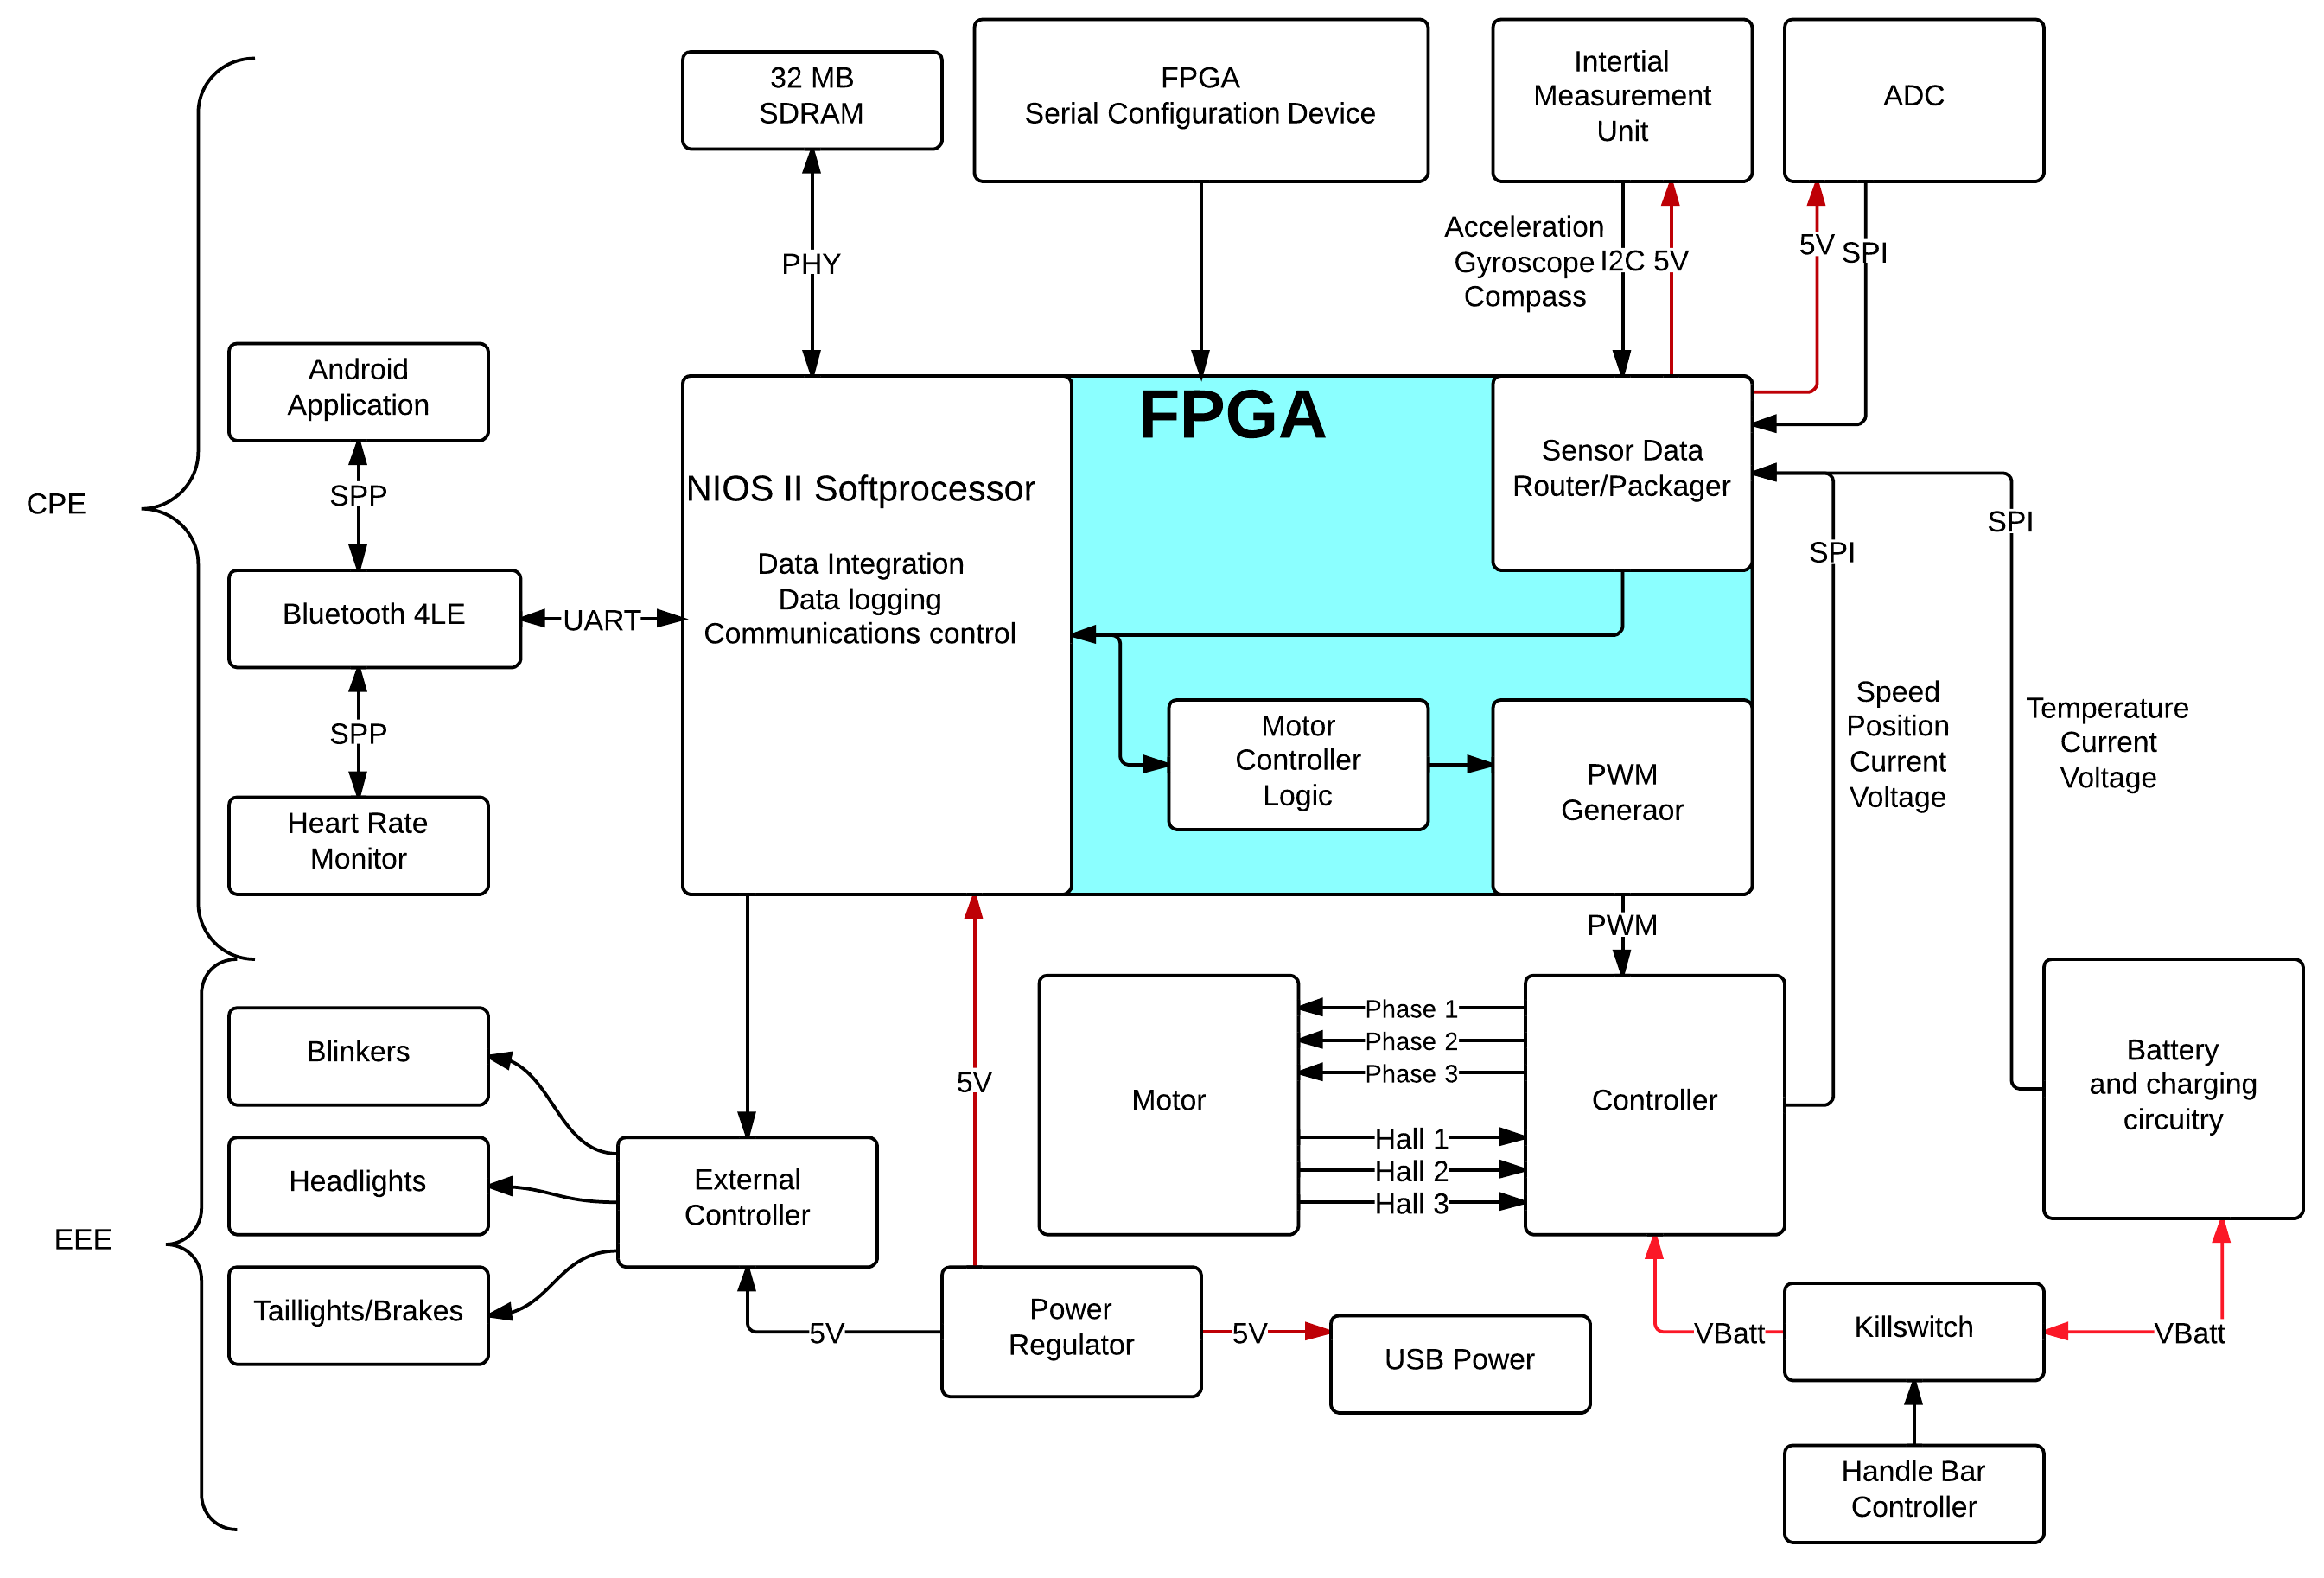
\includegraphics[width=\textwidth]{SystemDiagram}
        \caption{Block diagram of control hardware}
    \end{figure*}
    
%| Smart Assist 
%| ===========================================================s======================================
    \subsection{\bfseries Smart Assist}
            The amount of motor assist will be controllable in real time. This combined with a micro controller 
            and sensors will allow motor response tailored to the users need. The motor will have four modes of operation.
        \begin{itemize}
        \item Constant “effort” via feedback loop (HRT or Torque) \hfill \\
            PI feedback control system based on exertion measurement
    
        \item Inclination based assistance \hfill \\
           Linear wattage response to change in gradient
    
        \item Constant speed mode \hfill \\
            PID based control based on speed sensor
    
        \item Constant Wattage mode \hfill \\
         Basic wattage setting with no digital control.
        \end{itemize}
        
            These modes offer the user a variety options that require the use of external sensors or not. The constant
            wattage mode will need to be selectable and controllable via physical buttons on the device. The rest of the
            modes will be controlled by the Android application over the bluetooth connection.
            
            The motor must also turn off when the brakes are applied. There are a number of systems that detect the application
            of the brakes. The signal line from these sensors will be run into the FPGA to turn the motor output signal on and off. 
            
            To implement the NIOS II soft processor and other HDL entities  we will use Altera’s Quartus 13sp1 development
            environment. The actual programming of the Soft Processor will take place in a separate development environment called
            Nios® II Software Build Tools for Eclipse Indigo. Development of the control system in expected to require significant 
            effort. The MicroC RTOS will be implemented on the NIOS processor to handle task scheduling on the NIOS core. 
    
        \paragraph{\bfseries Central Processor}
            We will be using the NIOS II soft processor implemented on an Altera Cyclone IV FPGA. During
            the breadboard phase will use the Terasic DE0-Nano development board. This would mainly be 
            used to communicate with peripherals through UART and Bluetooth. This would also package and 
            store user data in a useful manner onto an SD card to be uploaded to PC or smart phone. 
        
        \paragraph{\bfseries Heartrate Based Control}
            The Zephyr HxM uses the bluetooth SPP (slave) protocol to communicate. the RN-41 bluetooth module 
            we plan to use can communicate with the heart rate strap operating  in master mode. Adding this feature 
            will allow motor torque to be varied in near real time automatically based on the users need. An example 
            implementation would be to use the Android application UI to specify a heart rate ceiling. As the user approaches 
            the ceiling value the output wattage of the motor is increased to provide assistance. The downside 
            is a 10 to 20 second delay from increase in exertion and heart rate response. The benefit is we can 
            provide a feedback system without having to implement the mechanically complicated torque measurements. \cite{HxMAPI}

        \paragraph{\bfseries Referenced control systems}
            \subparagraph{An SOPC based Intelligent Bike}   
                The authors of this paper developed a system to monitor tire pressure and and gear selection
                the most novel portion of their implementation is the use of cellphone RF to indicate the
                presence of other riders. \cite{SOPCBike}
                
            \subparagraph{Applying Fuzzy Logic Control to an Electric Bicycle}
                This paper details the Author's control system based on inclination. A control system
                was built around the rotational speed of the rear wheel. This system generated a PWM
                signal using a Programmable System On Chip.\cite{FuzzyLogicControl}
    
        \paragraph{\bfseries Qualifications for success}
            Smart control can be tested by isolating a control variable and manipulating it while recording
            the systems output data. The control algorithms are to be developed in a simulation environment and
            tested against generated data. A successful match between theoretical and experimental data will
            validate the systems performance.
                
        \begin{table}[H]        
            \renewcommand{\arraystretch}{1.3}
                    \caption{Estimated Time for smART Control}
                    
                    \label{Estimated Time}
                    
                    \centering
                    \begin{tabular}{p{5.5cm}|p{2cm}}
                    \hline
                    \bfseries   Task                        & \bfseries Labor Hours                         \\
                    \hline\hline
                                SPI for ADC                 & 16                                            \\
                                I2C for IMU                 & 25                                            \\  
                                NIOS II Core in Quartus     & 8                                             \\  
                                MicroC OS for NIOS II       & 8                                            \\
                                Verilog PWM Generator       & 4                                             \\
                                Verilog Motor Control       & 60                                            \\  
                                Verilog Sensor Parser       & 10                                            \\  
                                \hline
                    \end{tabular}
            \end{table}

%| Motor and Motor Control
%| =================================================================================================
    \subsection{\bfseries Motor and Motor Control}
        \paragraph{\bfseries Motor Selection}
            Our motor shall be contained within the rear hub of the bicycle. Placing the motor in the rear 
            will ensure the greatest traction while climbing. Rear mounting also attaches the motor to the 
            sturdiest portion of the frame. We have chosen a brushless design due to their availability, 
            durability, and reliability. Unlike a brushed DC motor, brushless designs don’t have electrical 
            contacts in the moving portion which can get contaminated or wear out. The motor will additionally 
            have the traditional bicycle gearing attached. 

    
        \paragraph{\bfseries Speed Controller}
            The motor shall be initially driven using an off the shelf electronic speed controller. This speed
            controller will accept a pulse width modulated signal generated by our master control unit and convert
            the the incoming signal to a 3 phase signal to power the motor.

            We shall design our own ESC to control the motor using the same pwm signal, however we will be 
            creating our own design to get more data out to the master control unit while incorporating a 
            power supply to get power to our master control unit and auxiliary systems.

            The electronic speed controller shall use a microprocessor to trigger 6 MOSFETS to conduct current 
            to the motor windings. It shall process data to feed back to the control unit. Ideally we would like 
            rotational speed, temperature, current, voltage, and torque data.

        \paragraph{\bfseries Qualifications for success}
            The motor will power the wheel to variable speed and power depending on the incoming signal, verified
            by an oscilloscope. The electronic speed controller shall detect wheel position and speed and control
            the motor to maintain a speed given an input signal.
            
       %|Estimated Hours of Work(Not Per Person)
       \begin{table}[H]        
            \renewcommand{\arraystretch}{1.3}
                \caption{Estimated Time for Speed Controller}
                
                \label{Estimated Time}
                
                \centering
                \begin{tabular}{p{5.5cm}|p{2cm}}
                \hline
                \bfseries   Task                        & \bfseries Labor Hours                         \\
                \hline\hline
                            Researching controllers     & 10                                            \\
                            Installing controller       & 4                                            \\  
                            Controller Design           & 90		\\
                            Motor Selection             & 8                                             \\
                            Installing Motor            & 5                                             \\  
                            Testing                     & 4                                             \\   
                            \hline
                \end{tabular}
        \end{table}

%| Power Distribution
%| =================================================================================================
    \subsection{\bfseries Power Distribution}
        \paragraph{\bfseries USB power}
            This will be a hub that will supply power and operate the various external functions of the 
            project including the lighting and sound. Additional slots will be added providing power for 
            whatever USB device the user chooses.  The main purpose for the extra slots are for charging a 
            cell phone which the user would use to adjust settings. This hub would provide six female USB 
            slots; four of these would be controlled by the FPGA and the other two would be always powered.
            The four controlled ports would be used for the lights and sound. The hub will take power from 
            the battery and step down the voltage to 5V and limit the current to 700mA for each output. The
            hub will also supply the power to the FPGA.

        \paragraph{\bfseries Qualifications for success}
        The ports must all produce 5V and the designated ports must be activatable by the FPGA.
            
      
      
      %|Estimated Hours of Work(Not Per Person)
        \begin{table}[H]        
            \renewcommand{\arraystretch}{1.3}
                \caption{Expected time for power distrobution system}
                
                \label{Expected time for power distrobution system}
                
                \centering
                \begin{tabular}{p{5.5cm}|p{2cm}}
                \hline
                \bfseries   Task                        & \bfseries Labor Hours                         \\
                \hline\hline
                            Power Hub Design            & 10                                             \\
                            Hub Fabrication             & 14                                            \\  
                            \hline  
                \end{tabular}
        \end{table}
        
%| Safety and Lighting
%| =================================================================================================
    \subsection{\bfseries Safety and Lighting}
        \paragraph{\bfseries Motor Safety}
            A number of safety systems need to be considered in the development of the control algorithm. All 
            operation modes must have a speed limit of 25 mph in accordance with state law. Accelerometer data 
            can be utilized to ensure the rider is upright and disable the drive motor in the event of a fall 
            for an added measure of safety. 
    
            A hard kill switch is to be between the battery and motor, this relay is to be held closed by the NIOS 
            soft processor. The signal line is to be use a pulldown resistor to ensure the relay will open in the 
            event of a software failure. A physical handlebar switch should be also attached to the motor’s kill 
            system so the user can kill the motor without having to rely on the FPGA control system.
        
        \paragraph{\bfseries Battery Safety}
            The volatile lithium polymer will need to have it's operation monitored to deal with a
            number of conditions which can harm the battery or lead to catastrophic failure. A robust
            charging system will be needed to prevent the battery from harmful overcharge or undercharge
            conditions. Short circuit protection will be needed as lithium polymer batteries are specifically
            susceptible to damage from high current conditions. Temperature and charge control mechanisms
            can be built into the FPGA. 

        \paragraph{\bfseries Lighting}
            The lighting will consist of a headlight, brake light, and front and rear blinkers. The 
            headlight will illuminate the area in front of the bicycle in order to increase the riders 
            visibility and perceptibility.  The lighting must not interfere with a driver’s ability to 
            see and thus must not shine directly into a driver’s eyes.  LEDs will be the illuminator 
            because of their small viewing angle which allows them to have a concentrated beam of light 
            without the use of reflection and their low energy consumption.  Some number of LEDs are to
            stay illuminated at all times the bike is in operation to increase visibility to drivers.  
            The rest of the LEDs in the headlight, which will be used for  illuminating the road in 
            front of the rider, will be activated manually or through light detection to activate 
            automatically in dark areas.
        
            The blinkers will consist of lights mounted on the rear, and possible front, of either side of 
            the bicycle.  The left light flashes when the rider flips the toggle up and the right light 
            flashes when the toggle is down to indicate which direction the rider intends to turn.  Both 
            lights remain off when the toggle is in the center position.  Blinkers may be combined with the 
            brake lights to reduce number of  units.
            
            The brake and tail light will be a red light or set of lights will be on at all times the 
            vehicle is in operation at a reduced intensity.  When the rider squeezes the braking lever, 
            the brake lights will engage with full intensity to alert people behind that the rider is 
            slowing down significantly or stopping.
            
            This feature will not require any software to run and will only need simple hardware: resistors, 
            LEDs, wires, switches and maybe some others if different modes are to be hardwired.  
      
        \paragraph{\bfseries Qualifications for success}
           If the lights switch state when the user interacts with them through the physical controls or 
           through the app, we know the module is working properly. Driving lights must turn on any time the
           vehicle is powered.
     
     %|Estimated Hours of Work(Not Per Person)
        \begin{table}[H]        
            \renewcommand{\arraystretch}{1.3}
                \caption{Estimated Time for Lighting and Safety}
                
                \label{Estimated Time}
                
                \centering
                \begin{tabular}{p{5.5cm}|p{2cm}}
                \hline
                \bfseries   Task                        & \bfseries Labor Hours                         \\
                \hline\hline
                            Design Schematics           & 4                                             \\
                            Proto Wiring and Testing    & 2                                             \\  
                            Design Casings and Mount    & 3                                             \\  
                            Fabricate Lights            & 15                                            \\
                            Fabricating Control Unit    & 3                                             \\
                            FPGA Logic Module           & 1                                             \\  
                            \hline  
                \end{tabular}
        \end{table}
    
%| User Interface and Controls
%| =================================================================================================
    \subsection{\bfseries User Interface and Controls}
        \paragraph{\bfseries Cell Phone Application}
            The cellphone application will primarily act as the rider’s dashboard. It will display the 
            rider’s speed, heart rate, location, and state of the system including battery charge, rate 
            of discharge, distance to empty estimation and power mode. The app is meant to be used from 
            a cell phone mounted to the handlebars much like the commercially available gps systems. The
            application will communicate with the NIOS II through Bluetooth and store required data on the 
            SD card. 
            
            The user will also be able to change the power mode and alter the system settings from the
            application. This should be the only interface to the system that the rider has to worry about,
            besides a physical kill switch in case a reset is required.
            
            The implement this system we will use Nios® II Software Build Tools for Eclipse Indigo to program 
            the FPGA’s Bluetooth utility and use the Eclipse IDE with built-in Android Developer Tools and Android 
            SDK components for programming the cell phone application.
            
        \paragraph{\bfseries Handgrip Controls}
            It is important for the rider to have a physical way to shut off the system seperate from the cell 
            phone application. This will be implemented with a switch next to the hand grip connected to a relay 
            between the battery and the motor. 
            
            There will be a toggle for the blinkers on the same mount, so the rider can control them with their
            thumb. Any other simple controls will be housed here. 
            
        \paragraph{\bfseries Qualifications for success}
            We can test the data comming into the FPGA with either an osciliscope or Signal Tap, and compare it to the 
            incoming data and the outgoing comands on the cell phone. We will also check eaech of the files of stored 
            data often to make sure there are no descrepencies, and the format is correct. Once we can communicate with
            the FPGA and are confident the data is accurate we will consier the section complete.
            
        \begin{table}[H]        
            \renewcommand{\arraystretch}{1.3}
                \caption{Estimated Time for Cell Phone Integration}
                
                \label{Estimated Time}
                
                \centering
                \begin{tabular}{p{5.5cm}|p{2cm}}
                \hline
                \bfseries   Task                            & \bfseries Labor Hours                     \\
                \hline\hline
                            Application UI                  & 8                                         \\
                            Data Processing/Presentation    & 16                                         \\
                            Data Storage Procedure          & 6                                         \\  
                            NIOS II Bluetooth               & 8                                         \\  
                            Cell Phone App Bluetooth        & 8                                         \\
                            \hline                          
                \end{tabular}
        \end{table}

%| Estimation of Cost
%| =================================================================================================
\section{\bfseries Estimated Costs}
    \begin{table}[H]
        \renewcommand{\arraystretch}{1.3}
            \caption{Cost Estimation}
            
            \label{Team Hour Summary}
            
            \centering
            \begin{tabular}{p{3cm}|p{1.5cm}|p{3cm}}
            \hline
            \bfseries   Part                & \bfseries Cost in Dollars(\$) & \bfseries Purpose     \\
            \hline\hline
                        DE0-Nano            & 100                           &   Central Processor   \\
                        9 DOF IMU           & 100                           &   Orientation Sensors \\  
                        Bluetooth           & 50                            &   Communication       \\  
                        Electric Motor      & 150                           &   Propulsion          \\
                        Motor Controller    & 100                           &   PWM to Motor        \\
                        Battery             & 400                           &   Power               \\  
                        BT4 Heart Rate      & 70                            &   HR Monitering       \\  
                        Bicycle             & FREE                          &   Framework           \\
                        Cell Phone          & FREE                          &   UI/Controls         \\
                        Miscellaneous       & 75                            &   Framework           \\
                        TOTAL               & 1050                          &   N/A                 \\        
                        \hline
                        TOTAL +35\%         & 1417                          &   Room For Error      \\        
                        \hline
            \end{tabular}
        \end{table}
%| =================================================================================================
%| End of Main Document
%| =================================================================================================

%Places bibliography at bottom of text
\bibliographystyle{IEEEtran}
\bibliography{IEEEfull}

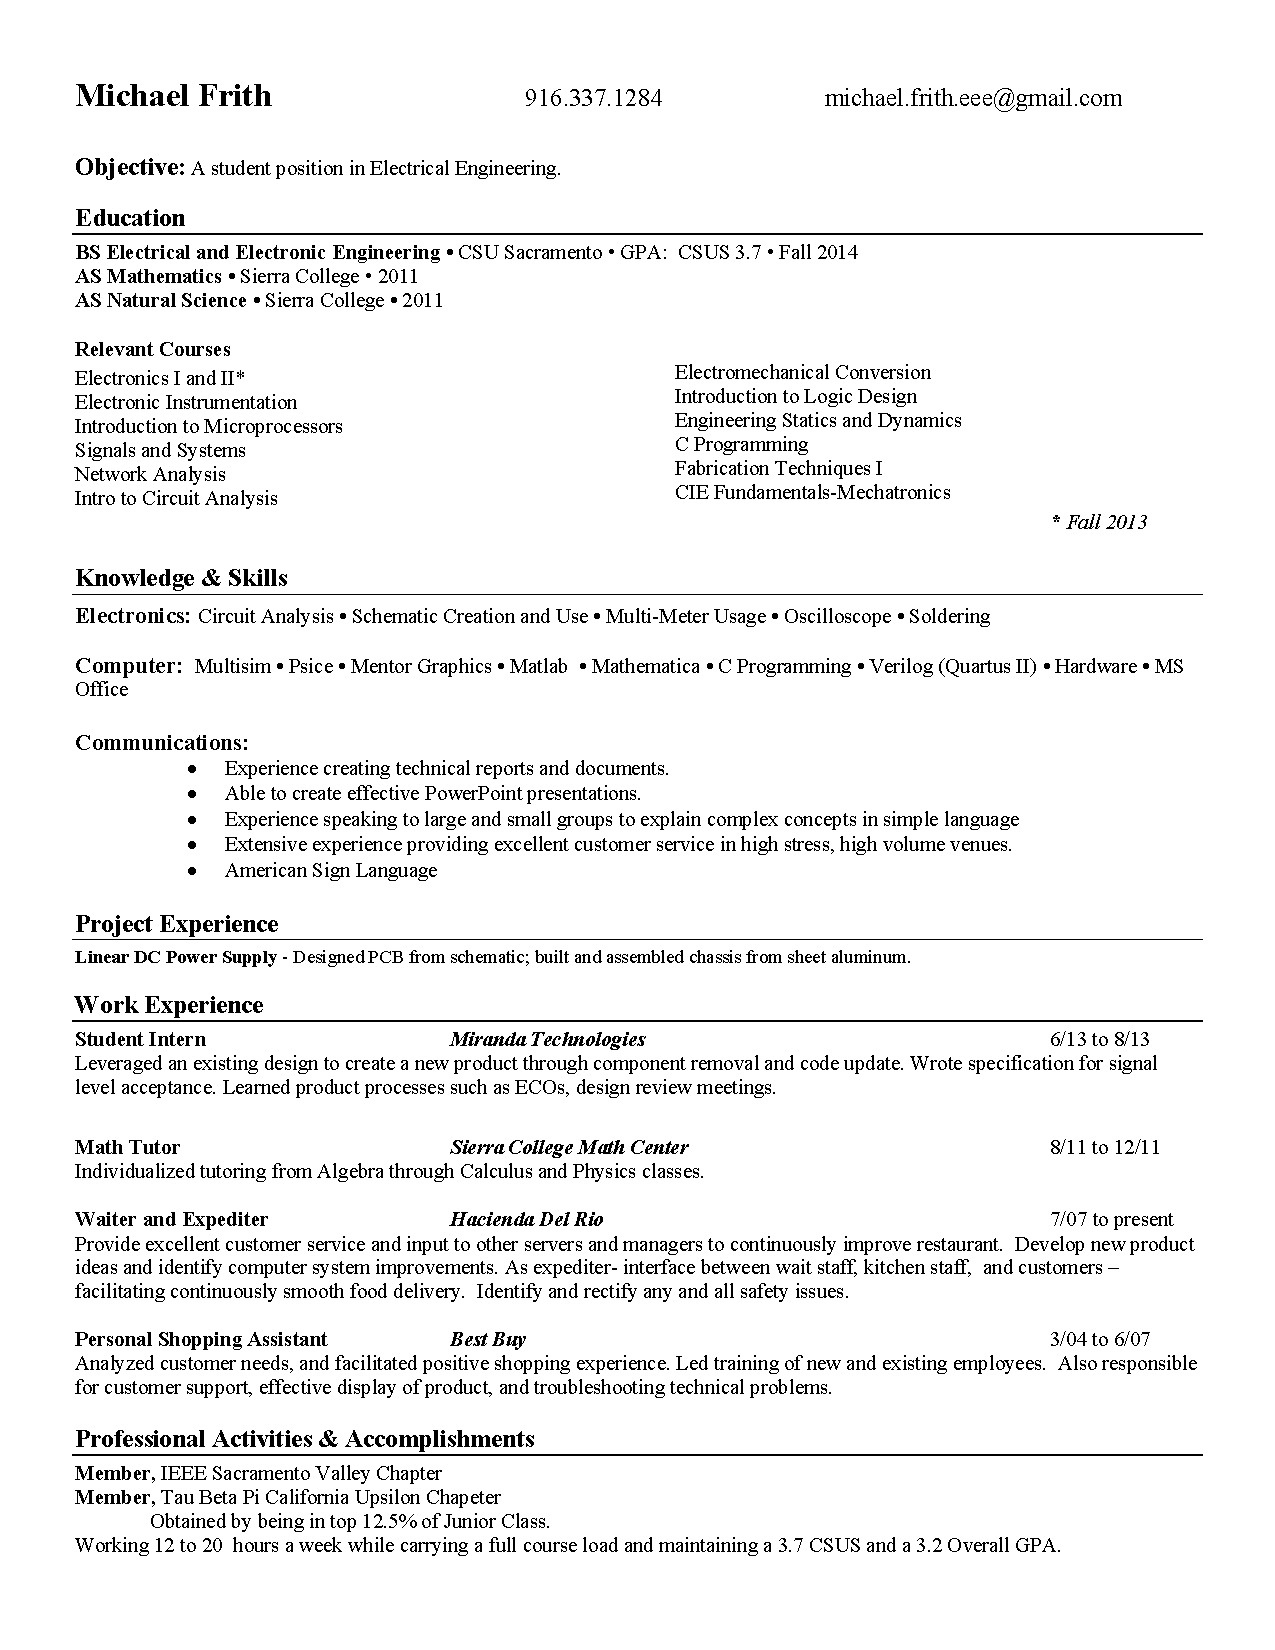
\includepdf{MikeFrith.pdf}
\includepdf{DavidLarribasResume.pdf}

\includepdf{DevinMooreResume.pdf}
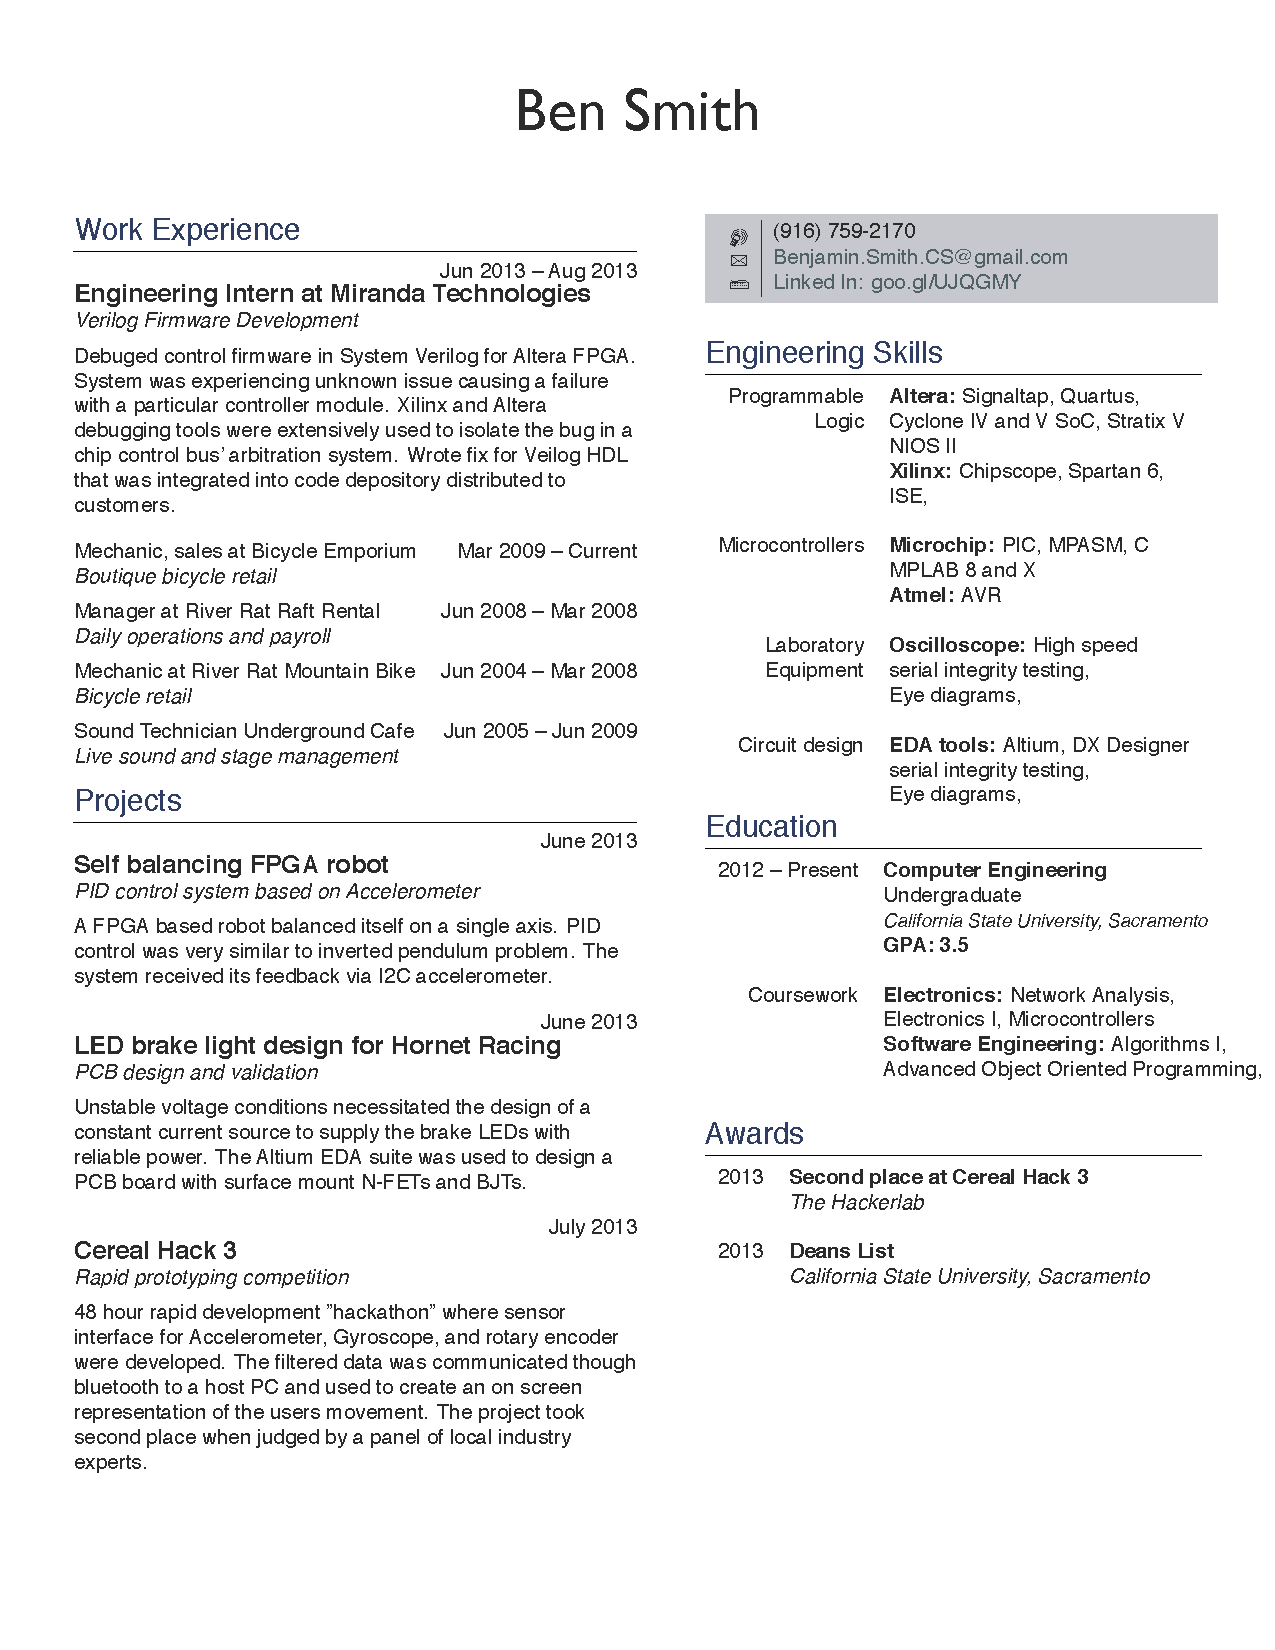
\includepdf{BenSmithResume.pdf}

\end{document}
